
\documentclass[12pt]{article}

\usepackage{physor2016}

\usepackage{amsmath}
\usepackage{bm}

\newcommand{\ve}[1]{\ensuremath{\mathbf{#1}}}
\newcommand{\Macro}{\ensuremath{\Sigma}}
\newcommand{\vOmega}{\ensuremath{\hat{\Omega}}}
\newcommand{\omvec}{\ensuremath{\hat{\Omega}}}
\newcommand{\rvec}{\ensuremath{\vec{r}}}
\newcommand{\vecr}{\ensuremath{\vec{r}}}

\usepackage{graphicx}
\usepackage{tikz}
\usepgflibrary{shapes.geometric}

\usepackage{booktabs}

\usepackage{siunitx}
%------------------------------------------------------------------------------

%------------------------------------------------------------------------------
% Define title. Use all CAPITALS.
%------------------------------------------------------------------------------
\title{FW/CADIS-$\Omega$: AN ANGLE-INFORMED HYBRID METHOD FOR DEEP-PENETRATION RADIATION TRANSPORT}
%
% ...and authors
%
\author{ 
  \textbf{Madicken Munk and R.~N.~Slaybaugh} \\
  Department of Nuclear Engineering, University of California, Berkeley \\
  3115B Etcheverry Hall, Berkeley, CA 94720, USA\\
  \href{mailto:madicken@berkeley.edu}{madicken@berkeley.edu}\\
  \href{mailto:slaybaugh@berkeley.edu}{slaybaugh@berkeley.edu}\\
  \\
  \textbf{Tara M.~Pandya, Seth R.~Johnson, and T.~M.~Evans}\\
  Radiation Transport Group\\
  Oak Ridge National Laboratory, P.O.\ Box 2008, Oak Ridge, TN 37831, USA\\
  \href{mailto:pandyatm@ornl.gov}{pandyatm@ornl.gov}\\
  \href{mailto:johnsonsr@ornl.gov}{johnsonsr@ornl.gov}\\
  \href{mailto:evanstm@ornl.gov}{evanstm@ornl.gov}
  }
  
%------------------------------------------------------------------------------
\renewcommand{\shortauthor}      % Author's names here
           {M.\ Munk~et~al.}  
\renewcommand{\shorttitle}       % Short title here
           {Angle-Informed CADIS and FW-CADIS}  

%------------------------------------------------------------------------------
% Setup PDF info. This sets several values which are listed as the "properties"
% of the PDF file.
%------------------------------------------------------------------------------
\hypersetup{
  pdftitle=\shorttitle,
  pdfauthor=\shortauthor
}


\begin{document}

%\doublespacing

%\linenumbers

%------------------------------------------------------------------------------
% Make the titlepage and set the pagestyle to fancy throughout
%------------------------------------------------------------------------------
\maketitle

\begin{abstract}
A new method for generating variance reduction parameters for strongly anisotropic, deep-penetration radiation shielding studies is presented. This method generates an alternate form of the adjoint scalar flux quantity, $\phi^{\dagger}_{\Omega}$, which is used by both CADIS and FW-CADIS to generate variance reduction parameters for local and global response functions, respectively. The new method, called CADIS-$\Omega$, was implemented in the Denovo/ADVANTG software suite, and results in a concrete labyrinth test problem are presented. Results indicate that the flux generated by CADIS-$\Omega$ incorporates localized angular anisotropies in the flux effectively. CADIS-$\Omega$ outperformed CADIS in the test problem while obtaining correct results. This initial work indicates that CADIS-$\Omega$ may be highly useful for shielding problems with strong angular anisotropies. A future test plan to fully characterize the new method is proposed, which should reveal more about the types of realistic problems for which the CADIS-$\Omega$ will be suited. 
\end{abstract}

\keywords{Hybrid Methods, CADIS, FW-CADIS, Angular Biasing}

%------------------------------------------------------------------------------
%
%------------------------------------------------------------------------------
\section{INTRODUCTION}
\label{sect::intro}

Efficiently modeling radiation transport in deep penetration shielding problems is essential to the safe operation of many types of nuclear facilities as well as the development of monitoring and detection systems. We would like to be able to perform such calculations with Monte Carlo (MC) methods, but it can be quite challenging to obtain acceptable statistical uncertainties in the computed tallies. Thus, many variance reduction (VR) strategies, some of which we will discuss, have been developed to facilitate accurate calculations in reasonable times. 

Problems that exhibit a strong degree of angular anisotropy in particle flux tend to be even more challenging for effective VR.
Many existing VR methods do not include angular information in their techniques, and therefore do not work well for these problems.  
Some VR methods do include angular information, but, in general, these methods have narrow applicability and/or are difficult to use and/or are computationally costly\textemdash rendering them inadequate as general tools.

With the goal of developing a method to easily, reliably, and inexpensively solve fixed-source problems that exhibit a high degree of angular anisotropy, we have developed a new method that builds on the Consistent Adjoint Driven Importance Sampling (CADIS) and Forward Weighted-CADIS (FW-CADIS) methods~\cite{wagner_forward-weighted_2007}, which we will jointly refer to FW/CADIS. 
%The new method builds on existing software infrastructure in a way that facilitates easy adoption.
FW/CADIS uses scalar flux estimates from a deterministic calculation to create VR parameters for use in MC.
Our new method uses a forward-weighted adjoint scalar flux based on a normalized contributon flux instead of a standard adjoint scalar flux, thereby including more angular information. 
We are calling the new method CADIS-$\Omega$, and FW/CADIS-$\Omega$ for both methods jointly.

We have implemented CADIS-$\Omega$ and tested it on an optically-thick source-detector labyrinth demonstration problem.
This demonstration problem has characteristics that are particularly challenging for existing VR methods and provides an opportunity to deeply investigate differences between this new method and CADIS.
We compare analog, standard CADIS, and CADIS-$\Omega$ calculations. 
Initial results show that for problems with strongly anisotropic behavior, CADIS-$\Omega$ outperforms traditional CADIS.

This paper begins with a background (Section~\ref{sect::second}) of important concepts relating to variance reduction and existing hybrid methods for deep-penetration radiation transport. 
We then provide the context of existing methods in Section~\ref{sect::past}. 
Section~\ref{sect::methodology} describes the mathematical foundation of our proposed method and the software that we used to implement it. 
The results and accompanying discussion are described in Section~\ref{sect::results}. Section~\ref{sect::future} presents our future test plans and details how this plan will characterize the application space beyond this single demonstration test. 
We conclude in Section~\ref{sect::conclusion}. 


%------------------------------------------------------------------------------
%
%------------------------------------------------------------------------------
\section{BACKGROUND}
\label{sect::second}
%
Many modern radiation transport codes offer variance reduction capabilities that employ an importance map\textemdash a measure of how important a particular region in a Monte Carlo simulation is to the tally being computed\textemdash to perform variance reduction. Generally, the importance of a cell can be defined as the ratio between the total score of particles entering the cell to the total weight of the cell \cite{booth_automatic_1982}. By generating an effective importance map for a system, the Monte Carlo calculation will have faster time to solution, a reduced variance, or both. 

Importance maps can be generated by a number of means, but a particularly effective method is to use the adjoint solution to the transport equation in the map creation. 
The solution to the adjoint equation has long been recognized as 
% What words did you want here? I'm putting in this to have something. 
% What you wrote is good. I like it. 
directly corresponding to how influential a given source particle will be on the defined as the adjoint source.
In fact, Kalos \cite{kalos_importance_1963, goertzel_monte_1958} and others have shown that an exact solution to the adjoint equation would result in a zero variance Monte Carlo solution. 

The steady state, fixed-source forms of the forward and adjoint transport equation are shown in Eqns.~\ref{eq:forward} and \ref{eq:adjoint}, respectively, where $\psi(\vec{r}, \hat{\Omega}, E)$ is the angular neutron flux, $\Sigma_t$ is the total macroscopic cross section, $\Sigma_s$ is the double-differential scattering cross section, $q$ is a fixed source, and superscript $\dagger$ indicates adjoint quantities.

\begin{align}
\bigl[\hat{\Omega} \cdot \nabla + \Macro_t(\vec{r}, E)\bigr] \psi(\vec{r}, \hat{\Omega}, E)  =  \int_0^{\infty} dE' &\int_{4\pi} d\hat{\Omega'} \:\Macro_{s}(\vec{r}, E' \to E, \hat{\Omega'} \cdot \hat{\Omega}) \psi(\vec{r}, \hat{\Omega'}, E')\nonumber \\
 &+ q(\vec{r}, \vOmega, E) \label{eq:forward} \\
%
\bigl[-\vOmega \cdot \nabla + \Sigma_t(\rvec, E)\bigr] \psi^{\dagger}(\vec{r}, \vOmega, E) = \int_0^{\infty} dE' &\int_{4\pi} d\vOmega' \: \Sigma_s(\rvec, E \rightarrow E', \vOmega \cdot \vOmega') \psi^{\dagger}(\rvec, \vOmega', E') \nonumber \\
&+ q^{\dagger}(\vec{r}, \vOmega, E) \label{eq:adjoint}
\end{align}

%In particular, the adjoint transport equation differs from the forward equation in that particles are scattered up in energy, from E to E', and are reversed in direction, from $\vOmega$ to $\vOmega'$. 
The key to using the adjoint flux for VR is defining the adjoint source~\cite{wagner_forward-weighted_2007}. 
Physically, $\psi$ represents how the source particles go forward and affect the rest of the problem space while $\psi^{\dagger}$ represents how the particles from a source come into the solution space and affect the answer. 
In this way, the angular adjoint flux represents how every part of phase space will influence the answer we are seeking.
%definition of the adjoint source, $q^{\dagger}$, depends on the nature of the problem being solved. 
For a simple source-detector problem, for example, $q^\dagger = \Sigma _{ d }$, the detector response function. 
%Thus, the adjoint particles start at low energy at the detector location, move away from the adjoint source (the detector location), and scatter up in energy. 

CADIS-$\Omega$ uses the contributon flux, the theory of which was pioneered by Williams~\cite{williams_generalized_1991,williams_contributorn_1992,williams_contributon_study}. 
The contributon flux is defined as
%
\begin{equation}
\Psi (\vec {r},\:\hat\Omega ,E) = \psi^{\dagger} (\vec {r},\:\hat\Omega ,E) \psi(\vec {r} ,\:\hat\Omega,E)\:.
\end{equation}
\label{eq.Cont-Flux} 
%
In contributon theory the pseudo-particle, called the \textit{contributon}, is a particle that carries ``response" from the radiation source to a detector. 
The contributon flux includes both forward and adjoint information, expressing the importance of a particle that is born at a forward source and as it move through space towards the detector, contributing to the solution.
In comparison, the adjoint flux exclusively places a high importance to particles which have a close proximity to the adjoint source. The direction from which these particles are likely to originate is not included in an adjoint-generated importance map.  Thus, an importance map founded on an adjoint flux will assign high importance to particles near the detector, no matter what direction they may be traveling. In contrast, an importance map generated by a contributon flux quantity will assign high importance to particles that are likely to be generated at the forward source and generate a response in the detector. 
% I do not understand this distinction as it is worded now...can you describe it more clearly?  
Becker's thesis~\cite{becker_hybrid_2009} aptly points out that this understanding of contributons is illustrated by a source-detector problem, where the forward source has little importance to the adjoint source, but does have importance to the problem solution.

Because contributons express response from the source to the detector, they can be useful for studies involving shield design and optimization. 
%Williams noted that variables relevant to contributon response were useful in determining transport paths through media~\cite{williams_contributon_study, williams_SCC_shielding}. 
%A study of the contributon density in a system could enlighten the user on locations where particles would preferentially be transported, and so designers could intelligently choose where to place detectors and material. 
%In this way, one could find the particles most influential to the response of the system. 
Contributon theory and spatial channel theory have been applied successfully to shielding analyses \cite{seydaliev_contributon_2008, williams_SCC_shielding} because they incorporate particle response throughout the entire system effectively. 
We are interested in the contributon flux because it finds preferential transport paths for particles that are born at the foward source and generate a response. This will have a strong effect on our variance reduction parameters, as the transport paths generated by the contributon flux will also allow for preferential transport paths in our adjusted Monte Carlo simulations. This will likely lead to a faster time to the solution, as less transport sampling will be performed in regions near the detector that are unlikely to have a source of forward source particles. 

%because they include angular information from both the forward and adjoint calculation. % Or some statement that is like this...I think clarifying above will help me understand how to state this. We don't want to talk about contributons as generally but to connect it to VR and this method.


\section{PAST WORK}
\label{sect::past}

The generation of an effective importance map is a key for a quality automated variance reduction technique. Both adjoint theory and contributon theory have been used to generate variance reduction parameters in deep-penetration radiation shielding problems. Perhaps the most widespread and accessible of these methods is the Consistent, Adjoint-Driven Importance Sampling (CADIS) method, which optimizes monte carlo transport for localized response functions by using 
Highlight the CADIS method \\
Highlight the FW-CADIS method \\
Talk about what problems CADIS and FW-CADIS succeed in, then talk about where they fall short. \\

Examples of variance reduction using importance maps include the weight window generator/weight window map (WWG) capability in the MCNP Monte Carlo code~\cite{brown_mcnp_2002}, and the FW/CADIS methods. Target weights in weight window maps are the inverse of the importance values for a given point in phase space.

For problems with very strong anisotropies in the particle flux, such as the streaming found near the air vents of an individual cask or in between casks stored in an array pattern, the importance map and biased source developed using the space/energy treatment above may not represent the real importance well enough to sufficiently accelerate the Monte Carlo calculation. Notice that the angular dependence of the importance function is not retained, because otherwise the map would be very large (tens or hundreds of GB) and more costly and complex to use in the Monte Carlo simulation. 

The drawback of this simplification is that, within a given space/energy cell, the map provides the average importance of a particle moving in any direction through the cell—excluding information about how particles move toward the objective. Consider the simple labyrinth example shown in Figure 1. For a source at the left entrance, the dose rate inside and outside of the labyrinth ranges over 12 orders of magnitude. Analog Monte Carlo would have to sample trillions of particles to get a few to the lowest dose regions. The space/energy treatment used in FW-CADIS makes this problem tractable but challenging. For particles near the turns in the labyrinth, the importance of the particles to the exit of the labyrinth vary greatly if they are coming out of a wall pointed toward the exit versus heading into a wall and away from the exit. This distinction is not captured by current hybrid methods. Including angular information in the importance map should significantly improve the Monte Carlo run time. 

Introduce angle-informed and angle-biased methods. \\
Higlight AVATAR + shortcomings \\
Highlight Turner \& Larsen's method + shortcomings\\

To do fast, accurate transport for used fuel monitoring, what is needed is an importance map generated quickly using deterministic methods that captures the impact of angle in the importance information. A variety of strategies for accomplishing this goal have been tried over the years. One such method is the Local Importance Function Transform (LIFT) method [10], which is derived from the zero-variance method and  uses an approximation of the adjoint flux that is piecewise continuous in angle. LIFT only captures linearly anisotropic scattering, which is not enough for our needs and is somewhat difficult to use [11].

More recently, an attempt by Peplow et al. [12] to solve this problem used the maximum entropy distribution [13] to approximate the angular adjoint flux, , and showed improvement in some problems but very little in others. In that work, the angular component of the adjoint flux was approximated as separable and symmetric about the average adjoint current direction. We will refer to this method as simple angular CADIS. Two versions were implemented, one with (limited) directional source biasing and one without. The method without source biasing is effectively the method used by the AVATAR [14] code on a Cartesian mesh and on a tet-mesh in a code by Evans and Wareing [13]. 

In Peplow et al.’s work, the improvement using simple angular CADIS over standard CADIS ranged from a factor of 0.09 to 3.3 over a collection of eight test problems, many of which have characteristics similar to used fuel cask monitoring systems. In all cases, CADIS and simple angular CADIS outperformed analog Monte Carlo. Peplow et al.’s study demonstrated that in many cases in which anisotropies are important, including angular information will improve calculation efficiency. However, these results also showed that the simple angular CADIS implementation is not accurate enough to provide the improvement necessary to be able to efficiently execute the used fuel cask calculations we would like to perform to improve facility monitoring design and operation. We therefore need to develop a better method for capturing the angular information.  
	


Conclude section with discussion of what is missing from CADIS/FW-CADIS/Angle Methods to motivate new method. \\

%------------------------------------------------------------------------------
%
%------------------------------------------------------------------------------
\section{METHODOLOGY}
\label{sect::methodology}

We have seen that past methods are challenged by problems with strong angular anisotropies or have limited use cases.
We build on past methods but calcualte the adjoint scalar flux in a way that has not been done before.
Using more angular information should deliver reliable, improved performance for problems in which angular information is particularly important. 
In this section we describe the theory behind the new method and why we believe it will work for highly anisotropic problems. We also present an overview of the software implementation.  

%------------------------------------------------------------------------------
%
%------------------------------------------------------------------------------
\subsection{Theory}
\label{subsect::theory}

Our new automated hybrid method incorporates angular information into the biasing parameters for FW/CADIS while not explicitly biasing in angle. 
That is, we generate space- and energy-dependent importance maps that incorporate the flux anisotropy in a more effective way than current implementations without adding the complication of angular weight windows. 
Both CADIS and FW-CADIS use an adjoint scalar flux to generate biasing parameters for variance reduction as shown in Eqns.~\eqref{}. 
FW/CADIS-$\Omega$ uses the same equations for weight windows and source biasing; what is different is how we create the adjoint flux. 
We weight the adjoint angular flux by the forward angular flux, integrate over angle, and divide by the integrated forward angular flux as shown in Eqn.~\eqref{eq:angularhybrid}.
This quantity, which we designate $\phi^{\dagger}_{\Omega}$, is then used in the FW/CADIS methods.
%
\begin{equation} 
\phi^{\dagger}_{\Omega}(\vec{r},E) = \frac{\int_{4\pi} \psi(\vec {r} ,E,\hat{\Omega})\psi^+(\vec {r} ,E,\hat{\Omega})d\hat\Omega }{\int_{4\pi}\psi(\vec {r} ,E,\hat{\Omega})d\hat\Omega}
\label{eq:angularhybrid}
\end{equation}

In a strongly anisotropic system, the adjoint scalar flux generated by Eqn.~\eqref{eq:angularhybrid} will be informed by what directions were most prominent in the forward case. 
Particles will be preferentially transported in the direction that they will actually be moving, rather than exclusively towards the adjoint source. 
This should allow for more effective Monte Carlo transport when angular effects are important. 
In an isotropic system, the $\phi^{\dagger}_{\Omega}$ will be essentially the same quantity as $\phi^{\dagger}$ generated in a deterministic adjoint simulation. 
% is that true?

We can also consider this method from another perspective: the contributon flux. 
The numerator of Eqn.~\eqref{eq:angularhybrid} is identified in the contributon flux, which, as described in Section \ref{sect::second}, represents the flux of response particles in a system. 
Contributons, then, are particles that will likely make it from the forward source to the detector to generate a response. 
%An importance map generated by the traditional adjoint scalar flux will differ significantly from a flux generated with a contributon flux. 
An importance map 
% Madicken -- I'm not really sure why you commented out everything here but left these three words? Do you want me to add to it? 
%from the adjoint flux will merely have greater importance with increasing proximity to the adjoint source, while the imporance map generated from 
%that includes the contributon flux will have strong importances in regions important to both the forward and adjoint angular fluxes. 
%
% 
%To calculate the quantity in eq. \eqref{eq:angularhybrid}, full angular flux maps of both the forward and adjoint problems will be required. 
%Further, an extra deterministic calculation (a forward calculation) will be required for CADIS-$\Omega$ calculations.

%------------------------------------------------------------------------------
%
%------------------------------------------------------------------------------

\subsection{Implementation}
\label{subsect::implementation}

We implemented the new method through the AutomateD VAriaNce reducTion Generator\\ (ADVANTG)~\cite{wagner_automated_2002, mosher_new_2010} software developed at ORNL. 
ADVANTG automates the generation of the importance map and biased source distribution created using either the CADIS or FW-CADIS methods for use in MCNP5~\cite{brown_mcnp_2002}. 
An input file in MCNP syntax is provided by the user in addition to some instructions for running ADVANTG. 
ADVANTG uses this information to exectue the discrete ordinates solver Denovo~\cite{evans_denovo:_2010} and uses the output to create the VR parameters for MCNP.
%The deterministic calculations can be performed using multiple cores and/or processors (e.g., on multi-core desktop systems and clusters). 
%ADVANTG takes Denovo's output, executes the CADIS or FW-CADIS methods, and the final variance reduction parameters are output in a format that can be used with unmodified versions of MCNP. 
%The primary objective of the development of ADVANTG has been to reduce both the user effort and the computational time required to obtain accurate and precise tally estimates across a broad range of challenging transport application areas.
The main reason we chose this system is the implementation is nearly invisible to the user and therefore the experience of using this method is nearly identical to using CADIS or FW-CADIS.
This facilitates easy adoption of software that is already easy to use.

%That is, the user simply adds an additional instruction asking to use the angle informed method and the interface does not change otherwise.
%Further, only one MCNP input file is required to compare the new method to FW/CADIS.
%Finally, it was simpler to implement the new method through ADVANTG than starting separately as we could take advantage of so much existing infrastructure in the coupling.

The major modifications required to implement this method were to Denovo. 
The angular flux is typically not stored or written by deterministic solvers as the desired output is typically the scalar flux.
The new method, however, requires both the forward and adjoint angular fluxes to create the scalar flux. 
Denovo therefore was modified to store and write the angular flux.
A new function was also added that performs the integration in Eqn.~\eqref{eq:angularhybrid}. 
This set of scalar fluxes is then written the same way as any scalar flux output from Denovo.

The benefit the bulk of the implementation being in Denovo is several fold. 
From the standpoint of ADVANTG, there are very few differences between the new method and FW/CADIS, making implementation is straightforward.
Further, anyone who finds a use for a scalar flux created as in Eqn.~\eqref{eq:angularhybrid} will now be able  access it.
Finally, it might be useful to have access to the full angular flux. 
Examining the angular flux for a problem could have research or pedagogical implications, and some other variance reduction method that uses the angular flux explicitly could be more easily developed in the future.

%------------------------------------------------------------------------------
%
%------------------------------------------------------------------------------
\section{RESULTS AND DISCUSSION} 
\label{sect::results}

% also address the ray effects differences between our method and CADIS
% change CADIS dots in response plots 
% Consider the detector response function for different energy neutrons. 
% Could put the detector response function on a dual axes for the response plot. 
% Talk about how well they perform relative to each other. 
%% This is what we did, this is what we saw, this is how we explain it. 

To begin to characterize the performance of CADIS-$\Omega$ we chose to study a candidate labyrinth source-detector test problem.
Such labyrinth problems contain some angle dependence that is not well captured by standard CADIS~\cite{Peplow-ORNL}. 
The motivation for these initial tests is to investigate the differences between CADIS and CADIS-$\Omega$. To identify and characterize this method with its classical counterparts, 
we will examine the adjoint scalar fluxes, which are effectively the importance maps, and the Monte Carlo figures of merit (FOMs) produced by each method, where 

\[\text{FOM} = \frac{1}{(\text{calculation time})*(\text{average relative error})^2}\:. \]

For the calculation of the FOM performed in this paper, the uncertainty in the tally total was used for $R$. 

We also performed an analog calculation with each geometry, comparing  the tally result, the relative uncertainty, and the FOM of the response tally (f4) for all three methods.
All methods used 10,000,000 particles, an f4 tally for the total reaction rate in the NaI detector, and energy bins matching the bounds of the library used by Denovo. 
The deterministic methods used the 27g19n shielding cross section library, a step characteristic (sc) spatial solver, quadruple range (qr) quadrature, a $P_N$ order of 2, and 135000 spatial cells. In ADVANTG, the quadruple range quadrature is set with four azimuthal and four polar angles per octant, and a default quadrature order of 10. 

Figure~\ref{fig::fwdflux} shows the problem geometry overlaid on a forward deterministic flux map. The labyrinth is comprised of a concrete shield, a 10MeV, isotropic point source at (-75, 0, 50), and a 10cm cubic NaI detector on the other side of the shield centered at (75, -15, 50). The edges of the problem have reflective boundary conditions, and the cross section libraries for MCNP were continuous energy. 

\begin{figure}
  \begin{center}
    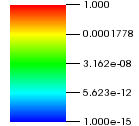
\includegraphics[width=0.10\textwidth]{./images/scale.png}
    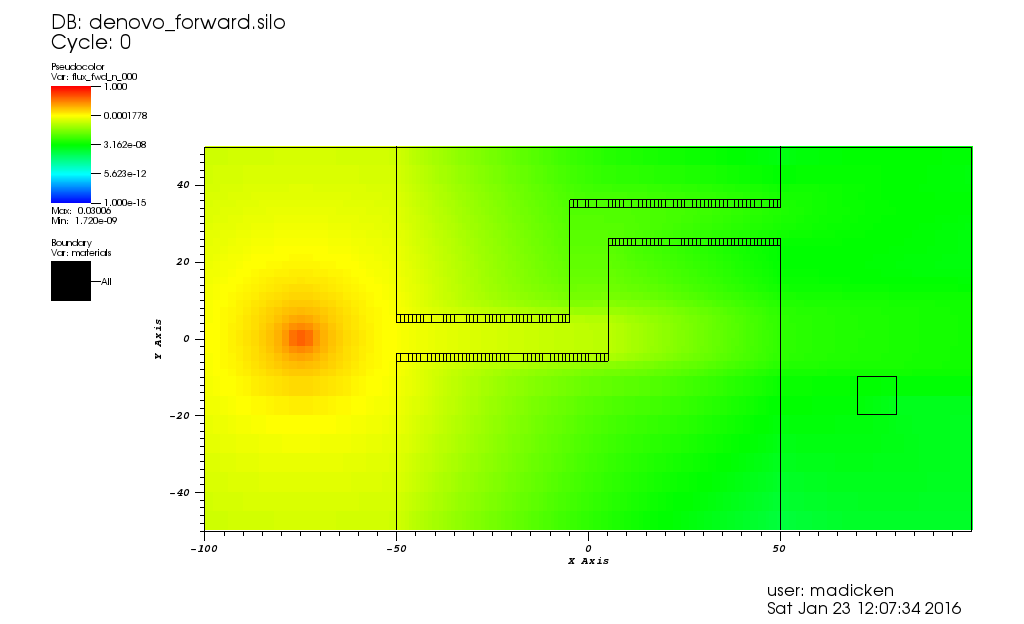
\includegraphics[width=0.80\textwidth]{./images/maze2_forward_group00_adjusted.png}
    \caption[]{\label{fig::fwdflux}Forward deterministic flux generated by Denovo for Labyrinth problem. Dimensions are in cm; the plots use the same color scale.}
  \end{center}
\end{figure}
% the axes and labels are really hard to read 

\begin{figure}
  \begin{center}
    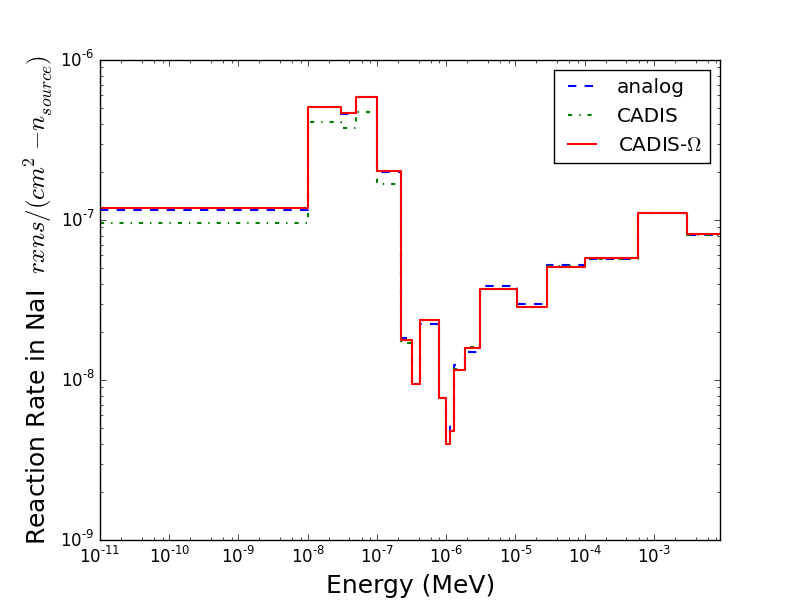
\includegraphics[width=0.49\textwidth]{./images/response.png}
    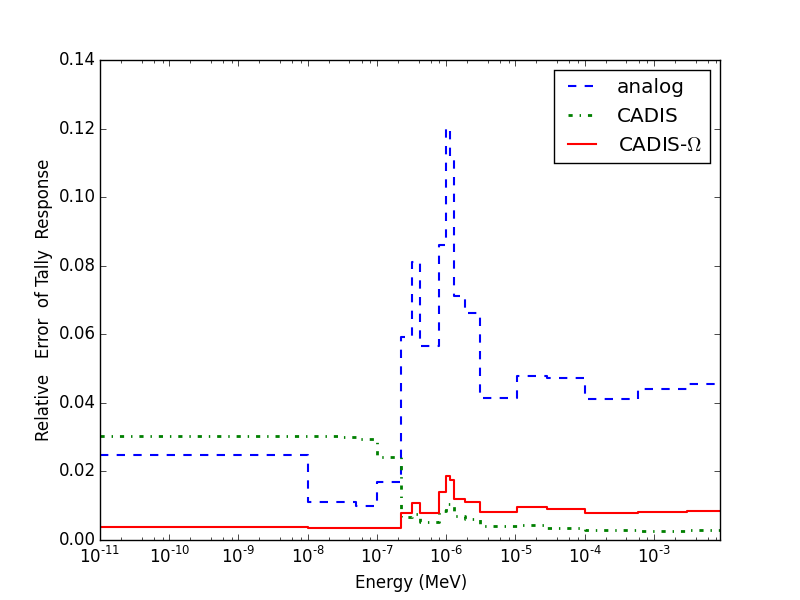
\includegraphics[width=0.49\textwidth]{./images/response_RE.png}
    \caption[]{\label{fig::tallyresponse} Responses (left) and relative uncertainties (right) in NaI detector tally for the Labyrinth problem. }
  \end{center}
\end{figure}
% Axes aren't great, hard to read the CADIS line
% These need error bars if possible, otherwise it is very difficult to compare


\begin{figure}
  \begin{center}
    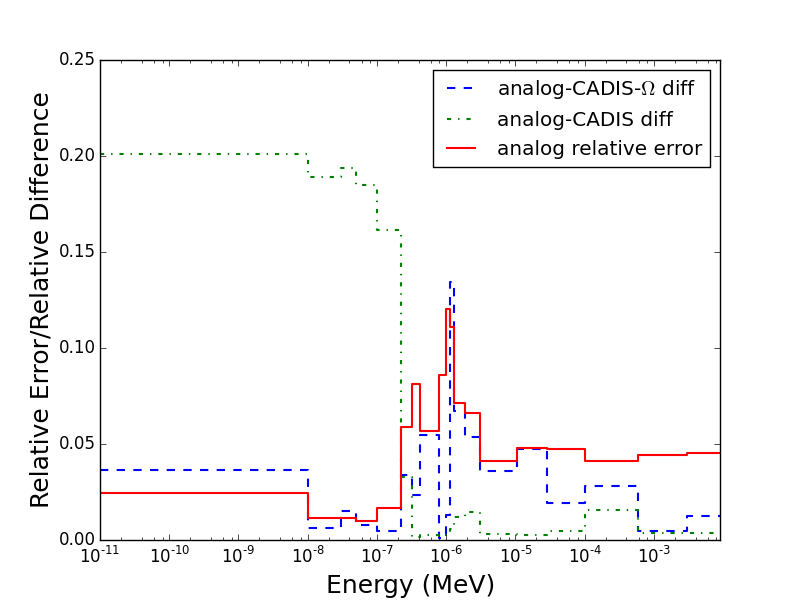
\includegraphics[width=0.49\textwidth]{./images/RE_differences.png}
    \caption[]{\label{fig::rediffs} Neutron flux at the NaI detector (left) and the sampled response function (right) that influence the detector response. }
  \end{center}
\end{figure}

\begin{figure}
  \begin{center}
    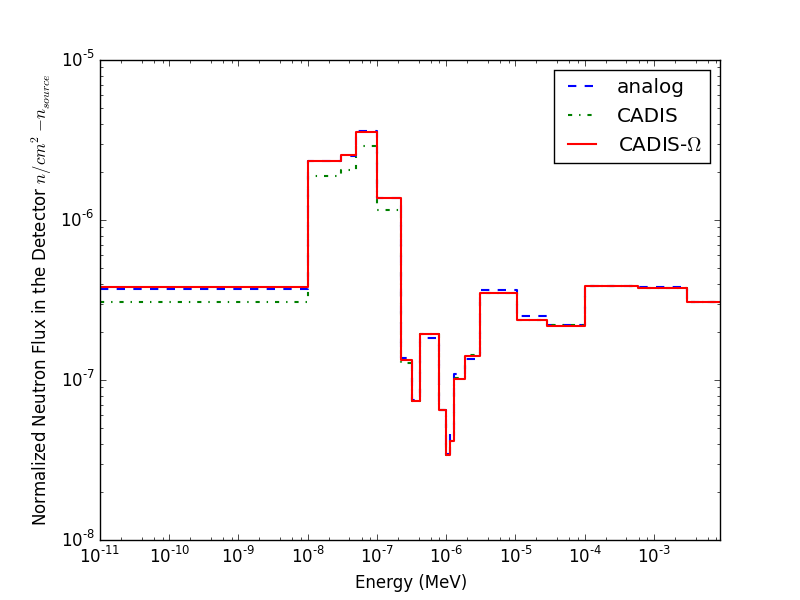
\includegraphics[width=0.49\textwidth]{./images/flux.png}
    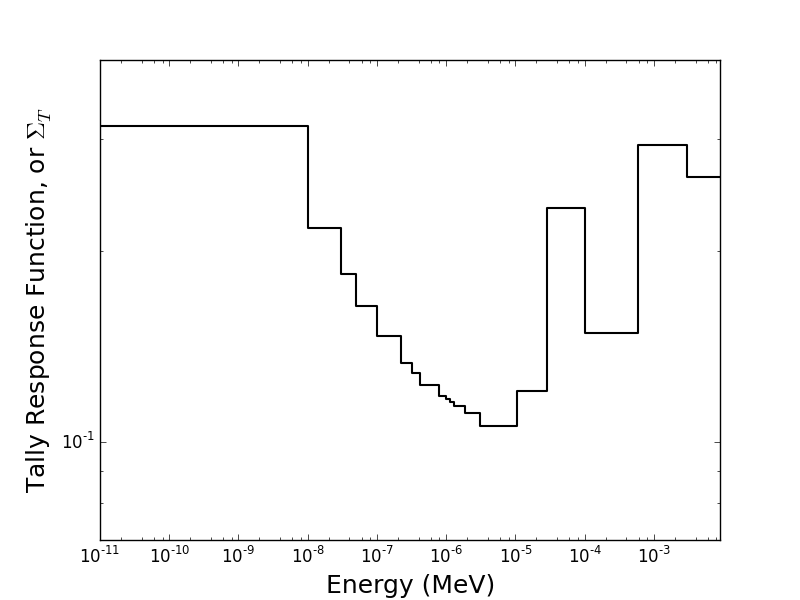
\includegraphics[width=0.49\textwidth]{./images/response_function.png}
    \caption[]{\label{fig::tallyproducts} Neutron flux at the NaI detector (left) and the sampled response function (right) that influence the detector response. }
  \end{center}
\end{figure}

The deterministic portion of the CADIS method took 57.4 minutes to solve and generate an output and CADIS-$\Omega$ took 116.44 minutes on a single core of a 3 GHz Intel Core i7 processor. The Monte Carlo runtimes for the analog, CADIS, and CADIS-$\Omega$ were 64, 386, and 367 minutes on a single, 20-core node of Intel Xeon E5-2670, resulting in FOMs of 493, 8.2, and 466, respectively.  In table \ref{tab:FOMLabI}, these results are summarized. In observing the adjusted FOM values, one should note that the system that performed the deterministic calculations was different than that of the Monte Carlo calculations. 

The tally responses and relative uncertainties for the NaI detector in the Labyrinth problem are shown in Figure~\ref{fig::tallyresponse} for the analog, CADIS, and CADIS-$\Omega$ methods.  CADIS-$\Omega$ has a lower relative error than CADIS for lower energy bins, but a higher relative error for higher energy bins. The relative error for CADIS-$\Omega$ appears to uniformly low. Comparatively, CADIS has the highest relative errors of all three methods at low neutron energies, but the lowest relative error for the highest energies. Not unsurprisingly, the analog response had the highest uncertainty in the lowest flux energy bins. Because adding error bars on the response plot of Figure~\ref{fig::tallyresponse} obscure the data, we have plotted the relative difference between CADIS and CADIS-$\Omega$ responses to the analog response in Figure~\ref{fig::rediffs}. For the most part, the responses are equivalent to within one standard deviation. This is not the case at low energies, where none of the methods lie within a standard deviation of each other, and CADIs lies well outside of the bounds of both the analog and CADIS-$\Omega$ methods. 

Separating the detector response into the flux and response function ($\Sigma_{T}$), as in Figure~\ref{fig::tallyproducts}, we can gain some insight as to why the low energy region is so problematic for these methods. Prior to 

The issues that lead to both CADIS and CADIS-$\Omega$'s disagreement with the analog calculation at low energies may be that they have not effectively sampled the intermediate energy range neutrons, which is a source for low energy neutrons. These neutrons have low importance to the detector response directly, the loss of their physics in the biasing schemes in CADIS and CADIS-$\Omega$ may be the source of this discrepancy, which merits further investigation. 

To investigate the reason that CADIS-$\Omega$ has higher relative error in some energies, we compared the adjoint flux distributions generated by CADIS and CADIS-$\Omega$ in a lower energy group, group 26 (1E-11 to 1E-08 MeV) and seen in Figure~\ref{fig::adjoint_fluxes_group26}, and a higher energy group, group 11 (2.9E-05 to 1.01E-04 MeV), and seen in Figure~\ref{fig::adjoint_fluxes_group11}.
Note that in these figures the color scales are not the same between groups so that the relative behavior of the flux within a method can be compared between the methods. It is the absolute difference between the flux values that will influence the weight window bounds, so this type of approach is reasonable. 

\begin{figure}
  \begin{center}
    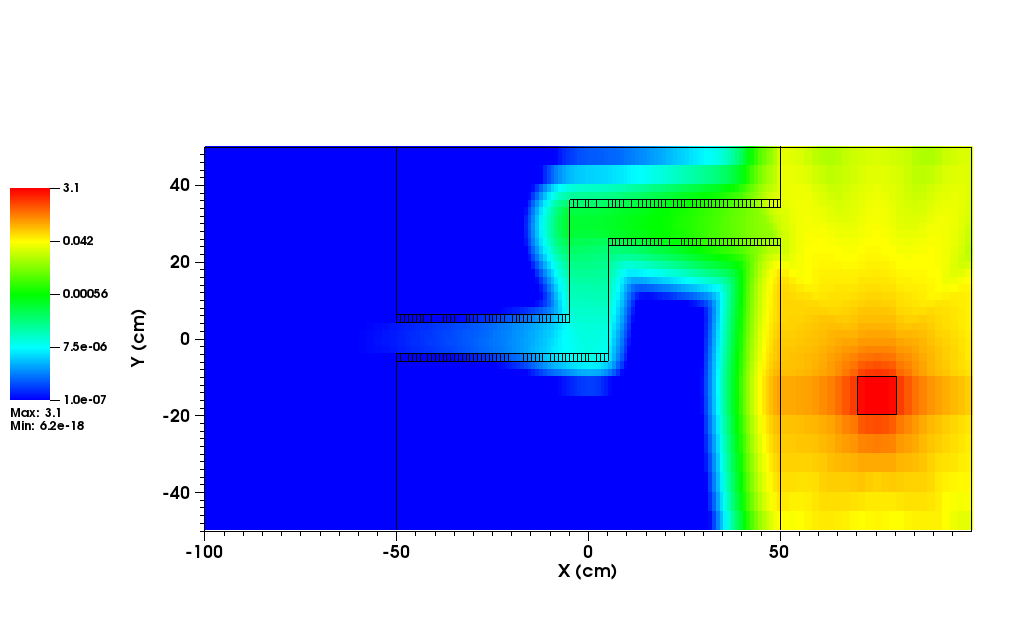
\includegraphics[width=0.80\textwidth]{./images/maze2_adjoint_group26_adjusted.png}
    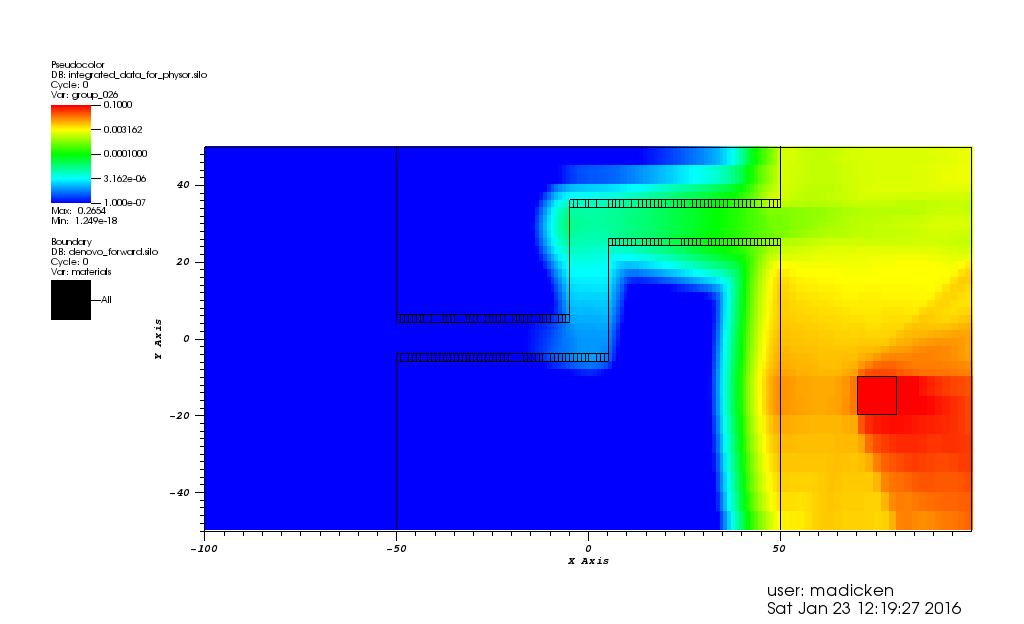
\includegraphics[width=0.80\textwidth]{./images/maze2_myflux_group26_adjusted.png}
    \caption[]{\label{fig::adjoint_fluxes_group26}\textit{Group 26} adjoint flux generated by standard Denovo (top) and CADIS-$\Omega$ method (bottom) for Labyrinth II geometry.}
  \end{center}
\end{figure}

\begin{figure}
  \begin{center}
    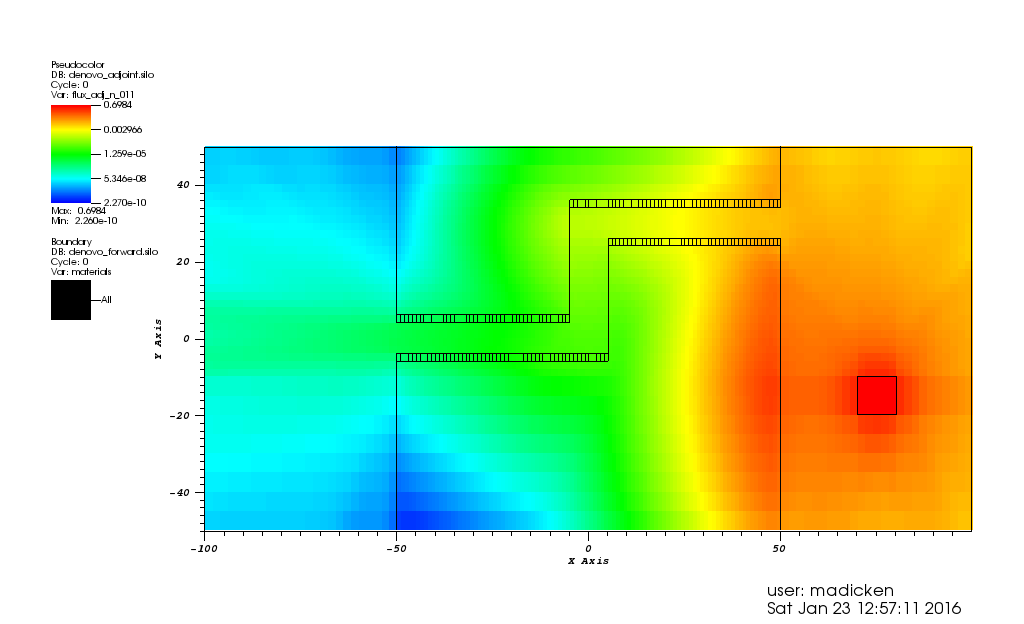
\includegraphics[width=0.80\textwidth]{./images/maze2_adjoint_group11_adjusted.png}
    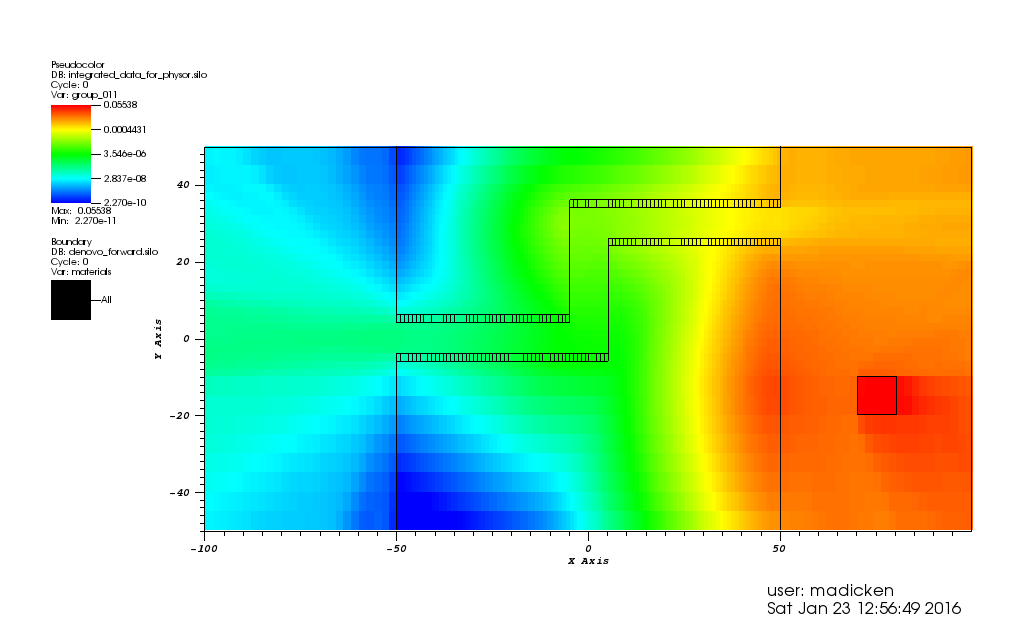
\includegraphics[width=0.80\textwidth]{./images/maze2_myflux_group11_adjusted.png}
    \caption[]{\label{fig::adjoint_fluxes_group11}\textit{Group 11} adjoint flux generated by standard Denovo (top) and CADIS-$\Omega$ method (bottom) for Labyrinth II geometry.}
  \end{center}
\end{figure}

In group 26, CADIS-$\Omega$ creates an adjoint flux in which the majority of the group 26 neutrons that contribute to the detector response are reflected off of the back and bottom walls, while the standard adjoint indicates fairly symmetric contribution. 
This illustrates that CADIS-$\Omega$ captures angular information differently than CADIS. 
We expect the shape of the CADIS map given the non-inclusion of angular information. 
The CADIS-$\Omega$ map seems to be strongly dominated by the reflecting behavior in the bottom right of the problem, indicating a more locally anisotropic behavior. This is likely due to the high probability of absorption of low energy neutrons in the shield. That is, low energy neutrons that are reflected off of the wall into the shield have a much lower survival probability than higher energy neutrons, like those in group 11. As a result, only the group 26 neutrons reflected directly towards the detector will contribute to the response, resulting in a locally anisotropic response-generating flux. 

This asymmetric effect in the CADIS-$\Omega$ case is not as prominent in group 11. 
Unlike group 26, the group 11 neutrons are far more likely to survive an interaction with the shield. As a result, the response-generating flux of group 11 has a similar probability to be from the reflective wall or the shield, resulting in a more locally-isotropic flux near the detector volume. This also has the effect that the group 11 CADIS-$\Omega$ adjoint fluxes more closely match the adjoint fluxes generated by CADIS. 
 
% MAKE SOME STATEMENTS ABOUT WHY THAT IMPACTS RELATIVE ERROR AND THE FOMs.\\
% Discuss differences and meaning of differences of results and parameter maps \\
% Discuss implications of these differences for solving other problems more generally 

 \begin{table}
  \centering
  \caption{\label{tab:FOMLabI}FOMs for Labyrinth Problem}
  \begin{tabular}{l|cc|cc}
    \toprule
    \hline
        & FOM$_{MC}$ & FOM$_{adjusted}$ & T$_{MC}$ (minutes) & T$_{determinstic}$ (minutes) \\
    \hline
    Analog           & 493   &  493     & 64.95      & 0.00 \\ 
    CADIS            & 8.2   &  7.1     & 386.18     & 57.4  \\
    CADIS-$\Omega$   & 466   &  353.88  & 367.42     & 116.4  \\  
	\bottomrule
  \end{tabular}
\end{table}


Table \ref{tab:FOMLabI} reports FOMs for both problems and all methods using the Monte Carlo simulation alone (designated MC), as well as an adjusted FOM that incorporates the runtimes for deterministic transport (designated adjusted). For a simple problem with the refined angular and spatial discretizations we chose, the deterministic calculation times were comparatively significant.
Because CADIS-$\Omega$ uses two deterministic transport calculations while CADIS uses one, incorporating the increased time for the calculation is necessary for a fair comparison.
It is worth noting that FW-CADIS-$\Omega$ and FW-CADIS would no longer have this discrepancy in deterministic calculation time.

The FOM's reported in Table \ref{tab:FOMLabI} reveal the significant effect that the high relative errors on low energy bin responses had on the FOM for CADIS. Because the low energy bins had a high response cross section in addition to a high flux, these bins strongly affected the FOM for CADIS. The strong difference in flux anisotropy near the deetector in Figure \ref{fig::adjoint_fluxes_group26} may also explain this. The biasing parameters generated by CADIS are encouraging the Monte Carlo calculation to spend equal calculation power to splitting and roulette on all sides of the source, even though the flux is most likely to reflect off of the wall to generate a response. As a result, CADIS spends more time tracking in regions with low contributing-particle density. This behavior wil allow CADIS-$\Omega$ to perform well for problems with a strong local anisotropy.  

Another important concept that will affect the succes of both CADIS and CADIS-$\Omega$ are ray effects, which are manifestations of rays in the flux that result from discretizing transport in the determinstic calculation. Both figures~\ref{fig::adjoint_fluxes_group26} and ~\ref{fig::adjoint_fluxes_group11} exhibit some ray effects behind the shield. Comparing the flux map between CADIS and  CADIS-$\Omega$,  CADIS-$\Omega$ does not seem to suffer any more from ray effects than traditional CADIS, and even appears to reduce them in some locations. This softening of the rays is a function of the integral performed in the numerator of eq. \eqref{eq:angularhybrid}. In the case of this problem, the streaming path out of the labyrinth is perpindicular to the rays generated by the adjoint source, which results in a softened adjoint-$\Omega$ flux map. However, a future problem where the ray effects in both the forward- and adjoint- sources lie parallel to one another might result in synergistic ray effects, which would have adverse effects on the variance reduction effectiveness of the $\Omega$-methods. The extent to which CADIS-$\Omega$ can reduce ray effects will be an important attribute to quantify in future studies.


Overall the performance of CADIS-$\Omega$ compared to CADIS and analog MC is promising. In our simple demonstration test problem, CADIS-$\Omega$ performed significantly better than CADIS by both FOM and relative error distribution inspection. CADIS-$\Omega$ had a more uniform uncertainty distribution in the response tally than both CADIS and the analog calculation. To determine the cause of these results, we compared the adjoint flux quantities calculated by CADIS and CADIS-$\Omega$. Inspection of the flux maps revealed that CADIS-$\Omega$ captures anisotropies in the flux, and these anisotropies are reflected in the variance reduction paramaters that are generated. Based on both theory and the method's performance in this demonstration problem, we expect that this method will perform well in problems with strong flux anisotropy generated by streaming paths or material heterogeneity, while performing poorly in problems with significant scattering effects where the flux may become more locally isotropic. 
 


%------------------------------------------------------------------------------
%
%------------------------------------------------------------------------------
\section{FUTURE WORK} 
\label{sect::future}
 
Section \ref{sect::results} showed that CADIS-$\Omega$ can outperform CADIS in a problem with a strong degree of angular anisotropy in the flux. However, there are a number of physical means by which angular anisotropy in the flux might occur. To further characterize the performance of CADIS-$\Omega$ and FW-CADIS-$\Omega$ throughout all of this physical phase space, we are planning to use a suite of test problems that should help quantify the performance of the method. The testing scheme identified in Table \ref{tab:testprobs} summarizes our testing plans. As noted in Section \ref{sect::results}, problems where the direction of particles is important to the importance of a cell are where we anticipate the strength to lie in CADIS-$\Omega$. These problems aim to address all of the physical means by which the flux could become strongly anisotropic, and some have shown to be difficult for traditional FW/CADIS~\citep{Peplow-ORNL}. The method's sensitivity to various determinstic discretization calculation parameters will also be investigated in these performance tests. 

 \begin{table}
  \centering
  \caption{Proposed Test Problem Coverage}
  \begin{tabular}{l|cccc}
    \toprule
    Problem Name & \multicolumn{4}{c}{Problem Coverage} \\
    \hline
     & Streaming Paths & High Scatter & Highly Heterog. & Beam Problem \\
    \hline
    Streaming Channel   & X & & & X \\ 
    Metal Plate         & X & X & X &  \\
    Labyrinth Variants  & X & X & X &  \\ 
    Spherical Boat      & X & & X & X \\  
    Kobayashi Benchmark & X & X &  &  \\   
	\bottomrule
  \end{tabular}
  \label{tab:testprobs}
\end{table}

After FW/CADIS-$\Omega$ has been fully characterized throughout the phase space identified in Table \ref{tab:testprobs}, it will be tested with large problems of interest. 
Specifically, we are interested in real problems that contain strong angular anisotropies that are difficult to solve, such as active interrogation problems, spent fuel cask storage (through air vents and between casks on ISFISIs), and facility calculations containing long gaps or streaming materials embedded in moderators. 
These large problem studies will be informed by the small problem studies and demonstrate the potential impact of this new method. 

%------------------------------------------------------------------------------
%
%------------------------------------------------------------------------------
\section{CONCLUSION} 
\label{sect::conclusion}

The existing state of fully automated hybrid methods does not have the ability to effectively capture angular anisotropies in the flux for effective variance reduction in deep-penetration radiation shielding problems. For problems that are strongly anisotropic, existing automated hybrid methods have poor performance, and do not produce results with the quality necessary to be used on a larger scale. There has been a strong push to remedy this in the hybrid methods community, but the methods that incorporate angular information for variance reduction are either not automated, not widely accessible, or are limited to particular anisotropic problem types due to assumptions in their methodology. 

We have presented and proposed a method, FW/CADIS-$\Omega$ that accesses the full energy- space- and angle- dependent angular fluxes from a deterministic calculation to generate a weighted form of the adjoint scalar flux. This weighted form of the adjoint flux is calculated by postprocessing the adjoint angular flux values from the discrete ordinates solver Denovo to pass a scalar flux value, $\phi^{\dagger}_{\Omega}$ to ADVANTG to use in CADIS and FW-CADIS. By using this scalar flux quantity, the weight windows generated by FW/CADIS-$\Omega$ will incorporate angular information without explicitly using angular biasing techniques. This method is based upon a strong theoretical foundation; it incorporates concepts from both adjoint and contributon theory. Because it has been implemented in large, production-level software, it will be easily accessible, and allow for fast adoption. 

We have explored the success of CADIS-$\Omega$ in a simple labyrinth test problem. This problem proved exceedingly difficult for CADIS, as it had a low FOM and lay outside of one standard deviation from the analog Monte Carlo problem. CADIS-$\Omega$ had a significantly higher FOM, a more uniform uncertainty distribution, and agreed well with the analog results. In comparing the flux quantity $\phi^{\dagger}$ and $\phi^{\dagger}_{\Omega}$ distributions over two energy groups, we found that CADIS-$\Omega$ generated dramatically different flux values in regions with strong local flux anisotropy. This is one of the contributing factors that explains CADIS-$\Omega$'s stronger performance for the example problem. While the example problem demonstrates the difference between CADIS and CADIS-$\Omega$, we have developed a comprehensive testing scheme that will help to characterize these methods. The testing phase of this project aims to (1) characterize the method's performance in a variety of problems that have anisotropies, and (2) demonstrate the method's applicability for large, realistic problems. 

% Recap what we told them (what problem we're trying to solve; about this method; how it's % different than past methods)\\
% Recap problem we solved and results\\
% Strong punchline paragraph about potential impact based on theory and these results.

FW/CADIS-$\Omega$ has yet to be fully characterized. The results from labyrinth I show that the $\phi^{\dagger}_{\Omega}$ captures local anisotropies in the flux, and this is reflected in the variance reduction parameters generated by FW/CADIS-$\Omega$.  Furthermore, the potential impact of creating a successful effective automated variance reduction parameters for problems with strong angular anisotropies in the flux are numerous. Large, site-level simulations with localized flux anisotropies will be solvable. Small, active-interrogation response functions can be quickly estimated at inspection stations. Shielding design and optimization will be quicker and faster. By  presenting, developing, characterizing, and testing FW/CADIS-$\Omega$, we are improving the understanding of how to incorporate angular information into variance reduction paramaters. 

%I'm not super happy with that last sentence, but I wasn't sure where to take it. I'll keep thinking about how to change it. 


%------------------------------------------------------------------------------
%
%------------------------------------------------------------------------------
\section*{ACKNOWLEDGMENTS}

This material is based on work supported by the Department of Energy under award number DE-NE0008286. This report was prepared as an account of work sponsored by an agency of the United States Government. Neither the United States Government nor any agency thereof, nor any of their employees, makes any warranty, express or implied, or assumes any legal liability or responsibility for the accuracy, completeness, or usefulness of any information, apparatus, product, or process disclosed, or represents that its use would not infringe privately owned rights. Reference herein to any specific commercial product, process, or service by trade name, trademark, manufacturer, or otherwise does not necessarily constitute or imply its endorsement, recommendation, or favoring by the United States Government or any agency thereof. The views and opinions of the authors expressed herein do not necessarily state or reflect those of the United States Government or any agency thereof.

\bibliographystyle{physor2016}
\bibliography{physor2016}

\appendix

\makeatletter
\def\@seccntformat#1{APPENDIX \csname the#1\endcsname.~}
\makeatother

%------------------------------------------------------------------------------
% If you need to make one (or more) appendix (appendices), place them here as
% sections
%------------------------------------------------------------------------------
\section{HOW TO MAKE APPENDICES}
\label{app::a}

This is a placeholder for my first appendix

\section{OTHER APPENDIX STUFF}
\label{app::b}

This is a placeholder for my second appendix

\end{document}

